\chapter{Results and Analysis\label{cha:results_analysis}}

The results chapter deals with presenting the different metrics discussed so far, within the RECAT-EU scheme. The data subset for the analysis was limited to four pair categories from the ICAO scheme: H-H, H-M, M-H and M-M. This simplification was done in order to filter out the small number of data points for other pairs, insufficient for any valid estimations of the distribution of inter-arrival distance or the landing time intervals. 

The distribution of inter-arrival distances for the RECAT-EU pairs were examined in agreement with the RECAT-EU reference separations. The AROT and LTI for particular pairs were compared to identify the limiting factor for throughput capacity, using the method already introduced in section LTI \fxnote{expoainagain how is lti and rot limiting. this secton comes later} .

\section{Aircraft Traffic Mix\label{sec:traffic_mix}}

The aircraft traffic mix is one of the components that affect runway capacity as mentioned in the Introduction section~\ref{sec:runway_capacity}. Analysing of the traffic mix outlines the main aircraft categories that will be considered for analysis, the portion of arrivals that will experience reduced wake turbulence separation minima along with estimate of the inter arrival distance characteristic of each pair. A simplified overview of the re-categorisation mechanism for BIKF is shown in Table~\ref{tab:wtc2recat_division}.

\begin{table}[h]
\centering
\resizebox{0.7\textwidth}{!}{%
\begin{tabular}{clcllc}
\multicolumn{3}{c}{\cellcolor[HTML]{34CDF9}HEAVY} &  &  & \cellcolor[HTML]{FD6864}LIGHT \\ \hline
\multicolumn{1}{|c|}{\cellcolor[HTML]{34CDF9}CAT-A} & \multicolumn{1}{c|}{\cellcolor[HTML]{34CDF9}CAT-B} & \multicolumn{1}{c|}{\cellcolor[HTML]{32CB00}CAT-C} & \multicolumn{1}{c|}{\cellcolor[HTML]{F8FF00}CAT-D} & \multicolumn{1}{c|}{\cellcolor[HTML]{F8FF00}CAT-E} & \multicolumn{1}{c|}{\cellcolor[HTML]{FFC702}CAT-F} \\ \hline
\multicolumn{1}{l}{} &  & \multicolumn{4}{c}{\cellcolor[HTML]{F8FF00}MEDIUM}
\end{tabular}%
}
\caption[Transition from ICAO WTC to RECAT-EU categories]{Transition from ICAO WTC to RECAT-EU categories. CAT-C combines aircraft from the ICAO Heavy and Medium categories and CAT-F combines aircraft from the Medium and Light categories. The categorisation process and criteria for assigning an existing aircraft type into RECAT-EU scheme is illustrated in detail in Figure~\ref{fig:RECAT_criteria}.}
\label{tab:wtc2recat_division}
\end{table}

Sorting the aircraft fleet arriving at BIKF into ICAO WTC reveals that the majority of flights~(85,4\%) are in the Medium wake category and the rest are mainly in the Heavy category~(14,2\%) with less than one percent Light aircraft~(Figure~\ref{fig:post_fast_exit_mix_pie_v2}). The small portion of Light flights can be explained with the policy of air traffic control at BIKF to avoid servicing those flights during the morning and afternoon peaks. This distribution of the three categories implies that combining the aircraft into arriving pairs would produce primarily Medium-Medium (M-M) pairs. This is confirmed later by the analysis of the number of arrival pairs in the ICAO categories (Table~\ref{tab:pairs_mix_to_wtc}).

\begin{figure}[h]
    \centering
    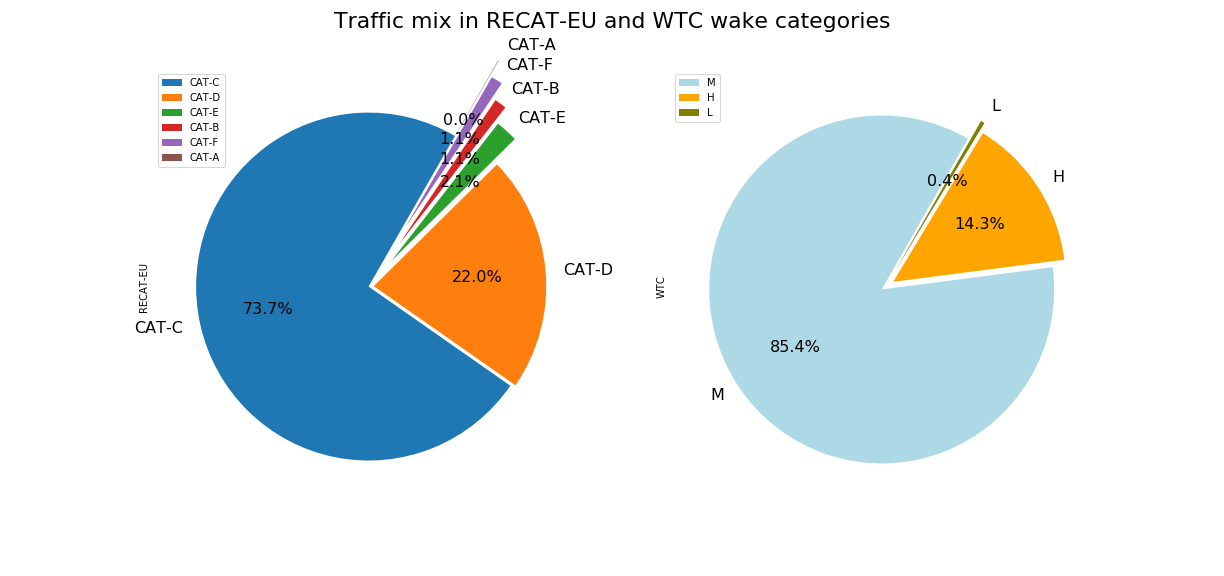
\includegraphics[width=1\textwidth]{graphics/fig_post_fast_exit_mix_pie_v2.png}
    \caption[Traffic mix in RECAT-EU and ICAO WTC]{The traffic mix at Keflavik Airport during peak hours, represented in RECAT-EU categories alongside ICAO WTC. The observed time period is 14 months starting October 2017.}
    \label{fig:post_fast_exit_mix_pie_v2}
\end{figure}

When this same fleet mix is presented using the RECAT-EU categories, the prevailing category is CAT-C (73,6\%), followed by CAT-D (22,1\%)~(Figure~\ref{fig:post_fast_exit_mix_pie_v2}). The percentage of each of the remaining categories varies but does not exceed 2\%. The expectation that this distribution of the RECAT-EU categories would result in primarily in C-C pairs is confirmed later on by the numbers presented in Table~\ref{tab:pairs_mix_to_recat}. 

Another approach for classification of the traffic fleet mix at BIKF during peak hours was to identify the aircraft types or models. The traffic data contains ICAO aircraft type designator, which is a two-, three- or four-character code composed of numbers and letters. This designator is unique for each aircraft type. The top fifteen aircraft types of the aircraft mix with their ICAO and RECAT-EU categories are presented in Figure~\ref{fig:traffic_mix_by_model}. Dominating the scene (56,8\% of all arrivals during peak hours) is the Boeing~757-200 model (ICAO: B752), followed by the Boeing~767-300 (ICAO: B763).

\begin{figure}[h]
    \centering
    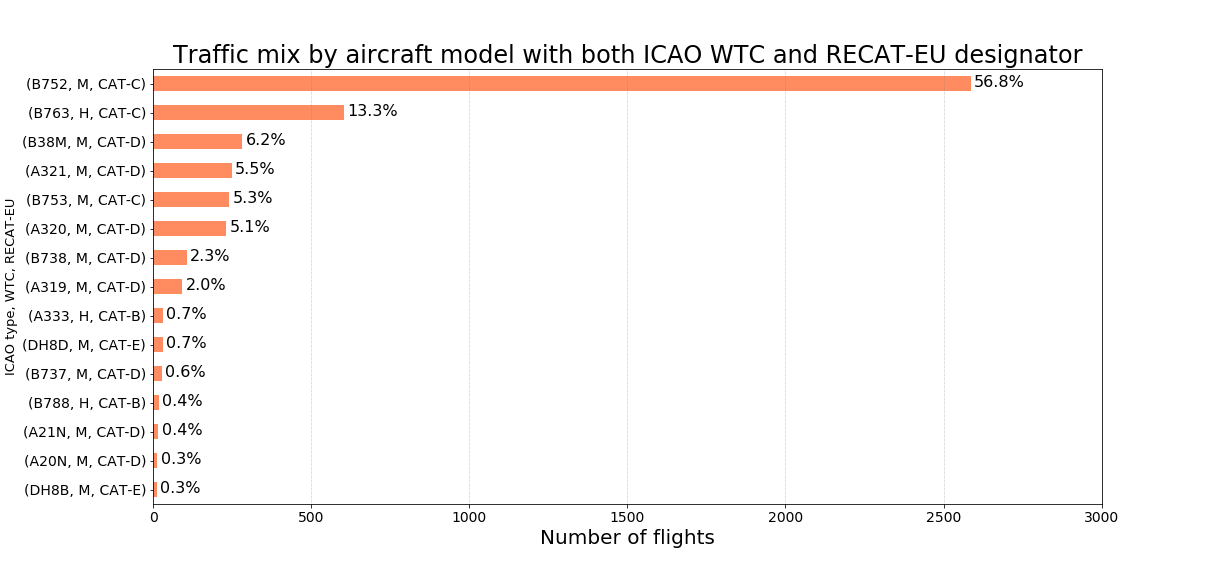
\includegraphics[width=1\textwidth]{graphics/fig_traffic_mix_by_model.png}
    \caption[Traffic mix by aircraft type.]{The traffic mix at Keflavik Airport during peak hours, grouped by aircraft type are shown alongside the ICAO WTC and RECAT-EU designators. The top three types comprise the major part of the Icelandair fleet. The observed time period is 14 months starting October 2017.}
    \label{fig:traffic_mix_by_model}
\end{figure}

 Those aircraft types represent a major part of the Icelandair fleet~\cite{icelandair_fleet} and the share of the Boeing~737~MAX~8 (ICAO: B38M) is likely to increase as the Icelandair company plans to gradually add sixteen new B38M and B39M models from the beginning of 2018. Flights operated by Icelandair for the observed period are 76.2\% of all arrivals during peak hours and 6,3\% of those are B38M flights. The tendency is towards increasing the share of the Medium WTC (or the CAT-D RECAT-EU category respectively), with the addition of the new aircraft to the Icelandair fleet.


\section{Arrival Runway Occupancy Time Considerations}\label{sec:AROT_considerations} 

\subsection{Traffic Mix and AROT\label{ssec:mix_effect_arot}}

Several approaches were used to look at the AROT at the airfield. First the runway occupancy was inspected based on the RECAT-EU category of the arrival aircraft in peak hours (Figure~\ref{fig:RECAT_AROTs_boxplot}).

\begin{figure}[h]
    \centering
    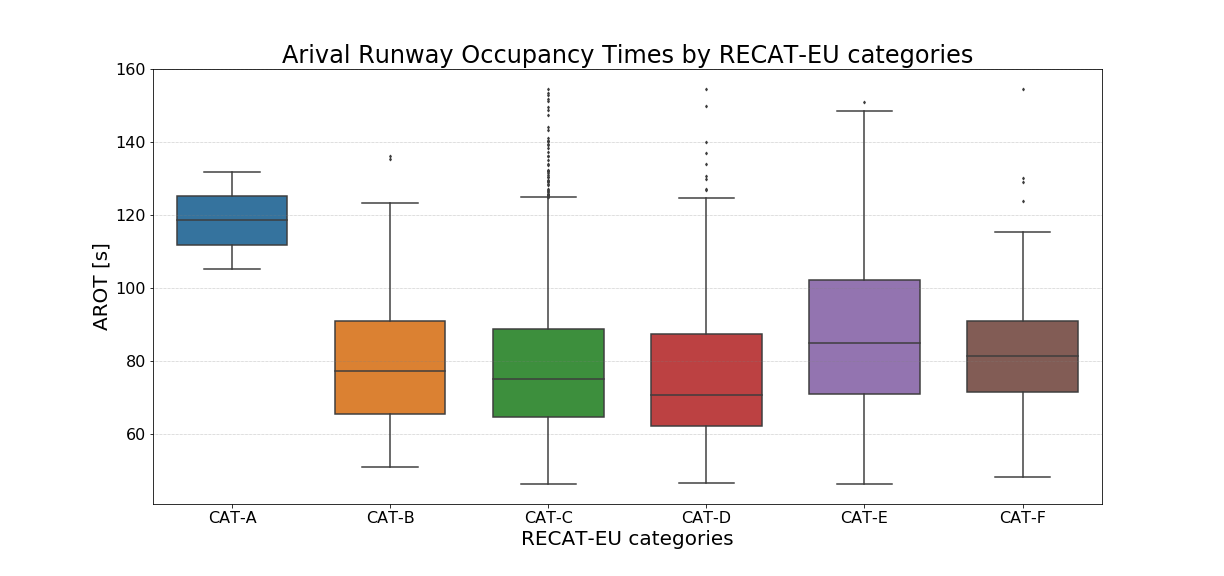
\includegraphics[width=1\textwidth]{graphics/fig_RECAT_AROTs_boxplot.png}
    \caption[AROTs box-plot for RECAT-EU categories, all runways]{Arrival Runway Occupancy Times for the different RECAT-EU categories based on data gathered for a period 14 months since October 2017. The coloured blocks indicate where 50\% of the data are located, or the inter-quartile range (IQR); lower edge is the 25\textsuperscript{th}~percentile (Q1), upper edge is the 75\textsuperscript{th}~percentile (Q3). The whiskers are at Q1-1,5$\times$IQR and Q3+1,5$\times$IQR.  The box plot shows the AROTs for all runways at BIKF during peak hours.}
    \label{fig:RECAT_AROTs_boxplot}
\end{figure}

The analysis showed that the shortest AROTs relate to aircraft from the CAT-D and CAT-C with mean values of 75 and 78 seconds respectively, as seen from the statistical analysis in (Table~\ref{tab:AROT_RECAT_stats}). These are also the two main categories that are considered in this study.

\begin{table}[h]
\centering
\resizebox{0.8\textwidth}{!}{%
\begin{tabular}{lr|r|r|r|r|r|r|r|}
\cline{3-9}
                          & \multicolumn{1}{c|}{}   & \multicolumn{7}{c|}{AROT [s]} \\ \hline
\multicolumn{1}{|l|}{RECAT-EU} & count & mean & std & min & 25\% & 50\% & 75\% & max \\ \hline
\multicolumn{1}{|l|}{CAT-A}    & 2     & 119  & 19  & 105 & 112  & 119  & 125  & 132 \\ \hline
\multicolumn{1}{|l|}{CAT-B}    & 53    & 81   & 20  & 51  & 65   & 77   & 91   & 136 \\ \hline
\multicolumn{1}{|l|}{CAT-C}    & 3447  & 78   & 17  & 46  & 65   & 75   & 89   & 155 \\ \hline
\multicolumn{1}{|l|}{CAT-D}    & 1034  & 75   & 18  & 46  & 62   & 71   & 87   & 155 \\ \hline
\multicolumn{1}{|l|}{CAT-E}    & 98   & 89   & 25  & 46  & 71   & 85   & 102  & 151 \\ \hline
\multicolumn{1}{|l|}{CAT-F}    & 49    & 83   & 22  & 48  & 72   & 81   & 91   & 155 \\ \hline
\end{tabular}%
}
\caption[AROTs for the air traffic mix by RECAT]{AROT statistics for the air traffic mix at BIKF by RECAT-EU categories. The count is the number of landings during peak hours since October 2017}
\label{tab:AROT_RECAT_stats}
\end{table}

The numbers also reveal that half of the aircraft from the CAT-C and CAT-D categories have AROTs in the range 60 to 90 seconds approximately, which outlines to some extent the anticipated values for AROT for the airfield. 

AROT is a metric that is expected to have minimal value, within certain safety limits, for increased throughput of the runway. One of the requirements for reducing the radar separation minimum (MRS) from 3~NM to 2,5~NM is AROT $\leq50$ seconds. ICAO Doc 4444 PANS-AM~\cite{doc44444} dictates that MSR may be reduced if the AROT of landing succeeding aircraft, which are established on the same final approach track is proven, by means such as data collection and statistical analysis and/or theoretical models, not to exceed 50 seconds. None of the average AROT values fulfils the 50~seconds limit for reduced MRS. This constraint fixes the MRS reference value at 3 NM and also suggest that the runway occupancy will be a limiting factor for the cases in which MRS is applicable (Table~\ref{tab:RECAT-dist}). This limitation is also confirmed by the statistical analysis for each of the runways in the following sections.% \ref{sssec:seasonal_arot}, \ref{sssec:runway_usage_arot}. 

\subsection{Seasonal Variation of AROT\label{ssec:seasonal_arot}}
Another approach was to analyse the seasonal variations of the runway occupancy time. The differentiation between summer and winter months was based on AROT values for a period of one year (Table~\ref{tab:month2season_arot}). Months with average AROT~$\leq$80~seconds formed the summer season and the rest were selected as winter months. This separation criteria is purely subjective but succeeds in forming two seasons with equal number of months. On average the seasonal difference of runway occupancy times was only eight seconds as seen in Table~\ref{tab:summer_winter_arot}. Still the seasonal variation should be taken into consideration as it can affect the AROT significantly, especially in the winter months when adverse weather conditions may impair the runway surface by accumulated slush, snow or ice, thus diminishing braking action. Good braking action due to runway surface condition is also one of the requirements for reduced MRS as provided by the procedures for navigation services of Air Traffic Management~\cite{doc44444}.

\begin{table}[h]
\centering
\resizebox{0.8\textwidth}{!} & \multicolumn{1}{l|}{50\%} & \multicolumn{1}{l|}{75\%} & \multicolumn{1}{l|}{max} \\ \hline
\multicolumn{1}{|l|}{SUMMER} & \multicolumn{1}{r|}{3727} & 76  & 17 & 46 & 63  & 72 & 87  & 155 \\ \hline
\multicolumn{1}{|l|}{WINTER} & \multicolumn{1}{r|}{956}  & 84  & 20 & 47 & 69  & 84 & 96  & 153 \\ \hline
\end{tabular}%
}
\caption[AROTs for the air traffic mix by season]{AROT statistics for the air traffic mix at BIKF by season. The count is the number of landings during peak hours over a 13 month period starting October 2017.}
\label{tab:summer_winter_arot}
\end{table}

\subsection{Runway Usage and AROT\label{ssec:runway_usage_arot}}
Runway occupancy for each of the runways was also examined both with regard to seasonal variations and rapid-exit taxiway usage. The usage of the four runways during peak hours is shown in Figure~\ref{fig:runway_usage_peak}. 

\begin{figure}[h]
    \centering
    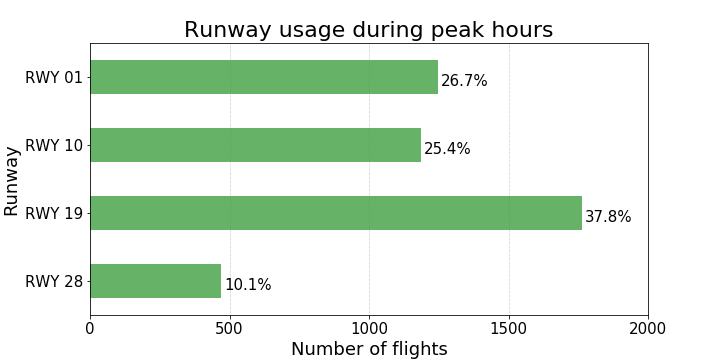
\includegraphics[width=0.8\textwidth]{graphics/fig_runway_usage_peak.png}
    \caption[Runway usage at BIKF during peak hours]{Runway usage at BIKF during peak hours for a period of 14 months starting October 2107. RWY-19 is the most frequently used runway, followed by RWY-01 and RWY-10. The RWY-01 is connected to rapid-exit TWY~A-1 and RWY-28 to rapid-exit TWY~B-1.}
    \label{fig:runway_usage_peak}
\end{figure}

BIKF airfield is currently equipped with two rapid-exit taxiways designated as TWY~A-1 and TWY~B-1. The first was completed on 26~July~2017 and the latter on 4~October~2017. The day that A-1 became operational was chosen as the starting time for the data set considered for analysis in this project. The reason behind this is the beneficial effect that rapid-exits have on reducing arrival runway occupancy time. Taxiway A-1 provides a rapid-exit track to the left for RWY-01, in the north landing direction, and B-1 serves RWY-28 exiting to the right in the west direction. The statistical analysis points to decreased AROT on average for RWY-01 after the start of A-1 (Table~\ref{tab:season_AROT_stats_RWY01_pre_fast_exit},~\ref{tab:season_AROT_stats_RWY01_post_fast_exit}). This decrease was primarily during the winter season (12 seconds) but trivial for the summer months. The data for RWY-28 presented a different picture. The average AROT has been reduced by 31 seconds for the summer months and by 37 seconds for the winter, after the implementation of the rapid-exit (Table~\ref{tab:season_AROT_stats_RWY28_pre_fast_exit},~\ref{tab:season_AROT_stats_RWY28_post_fast_exit}). The minor gain of RWY~01 with TWY~A-1 can be explained with its layout and the fact that A-1 exits into TWY~E-3, meeting taxiing aircraft in the opposite direction (Figure~\ref{fig:BIKF_schematic}), so the rapid-exit was avoided altogether during peak hours.

\begin{figure}[h]
    \centering
    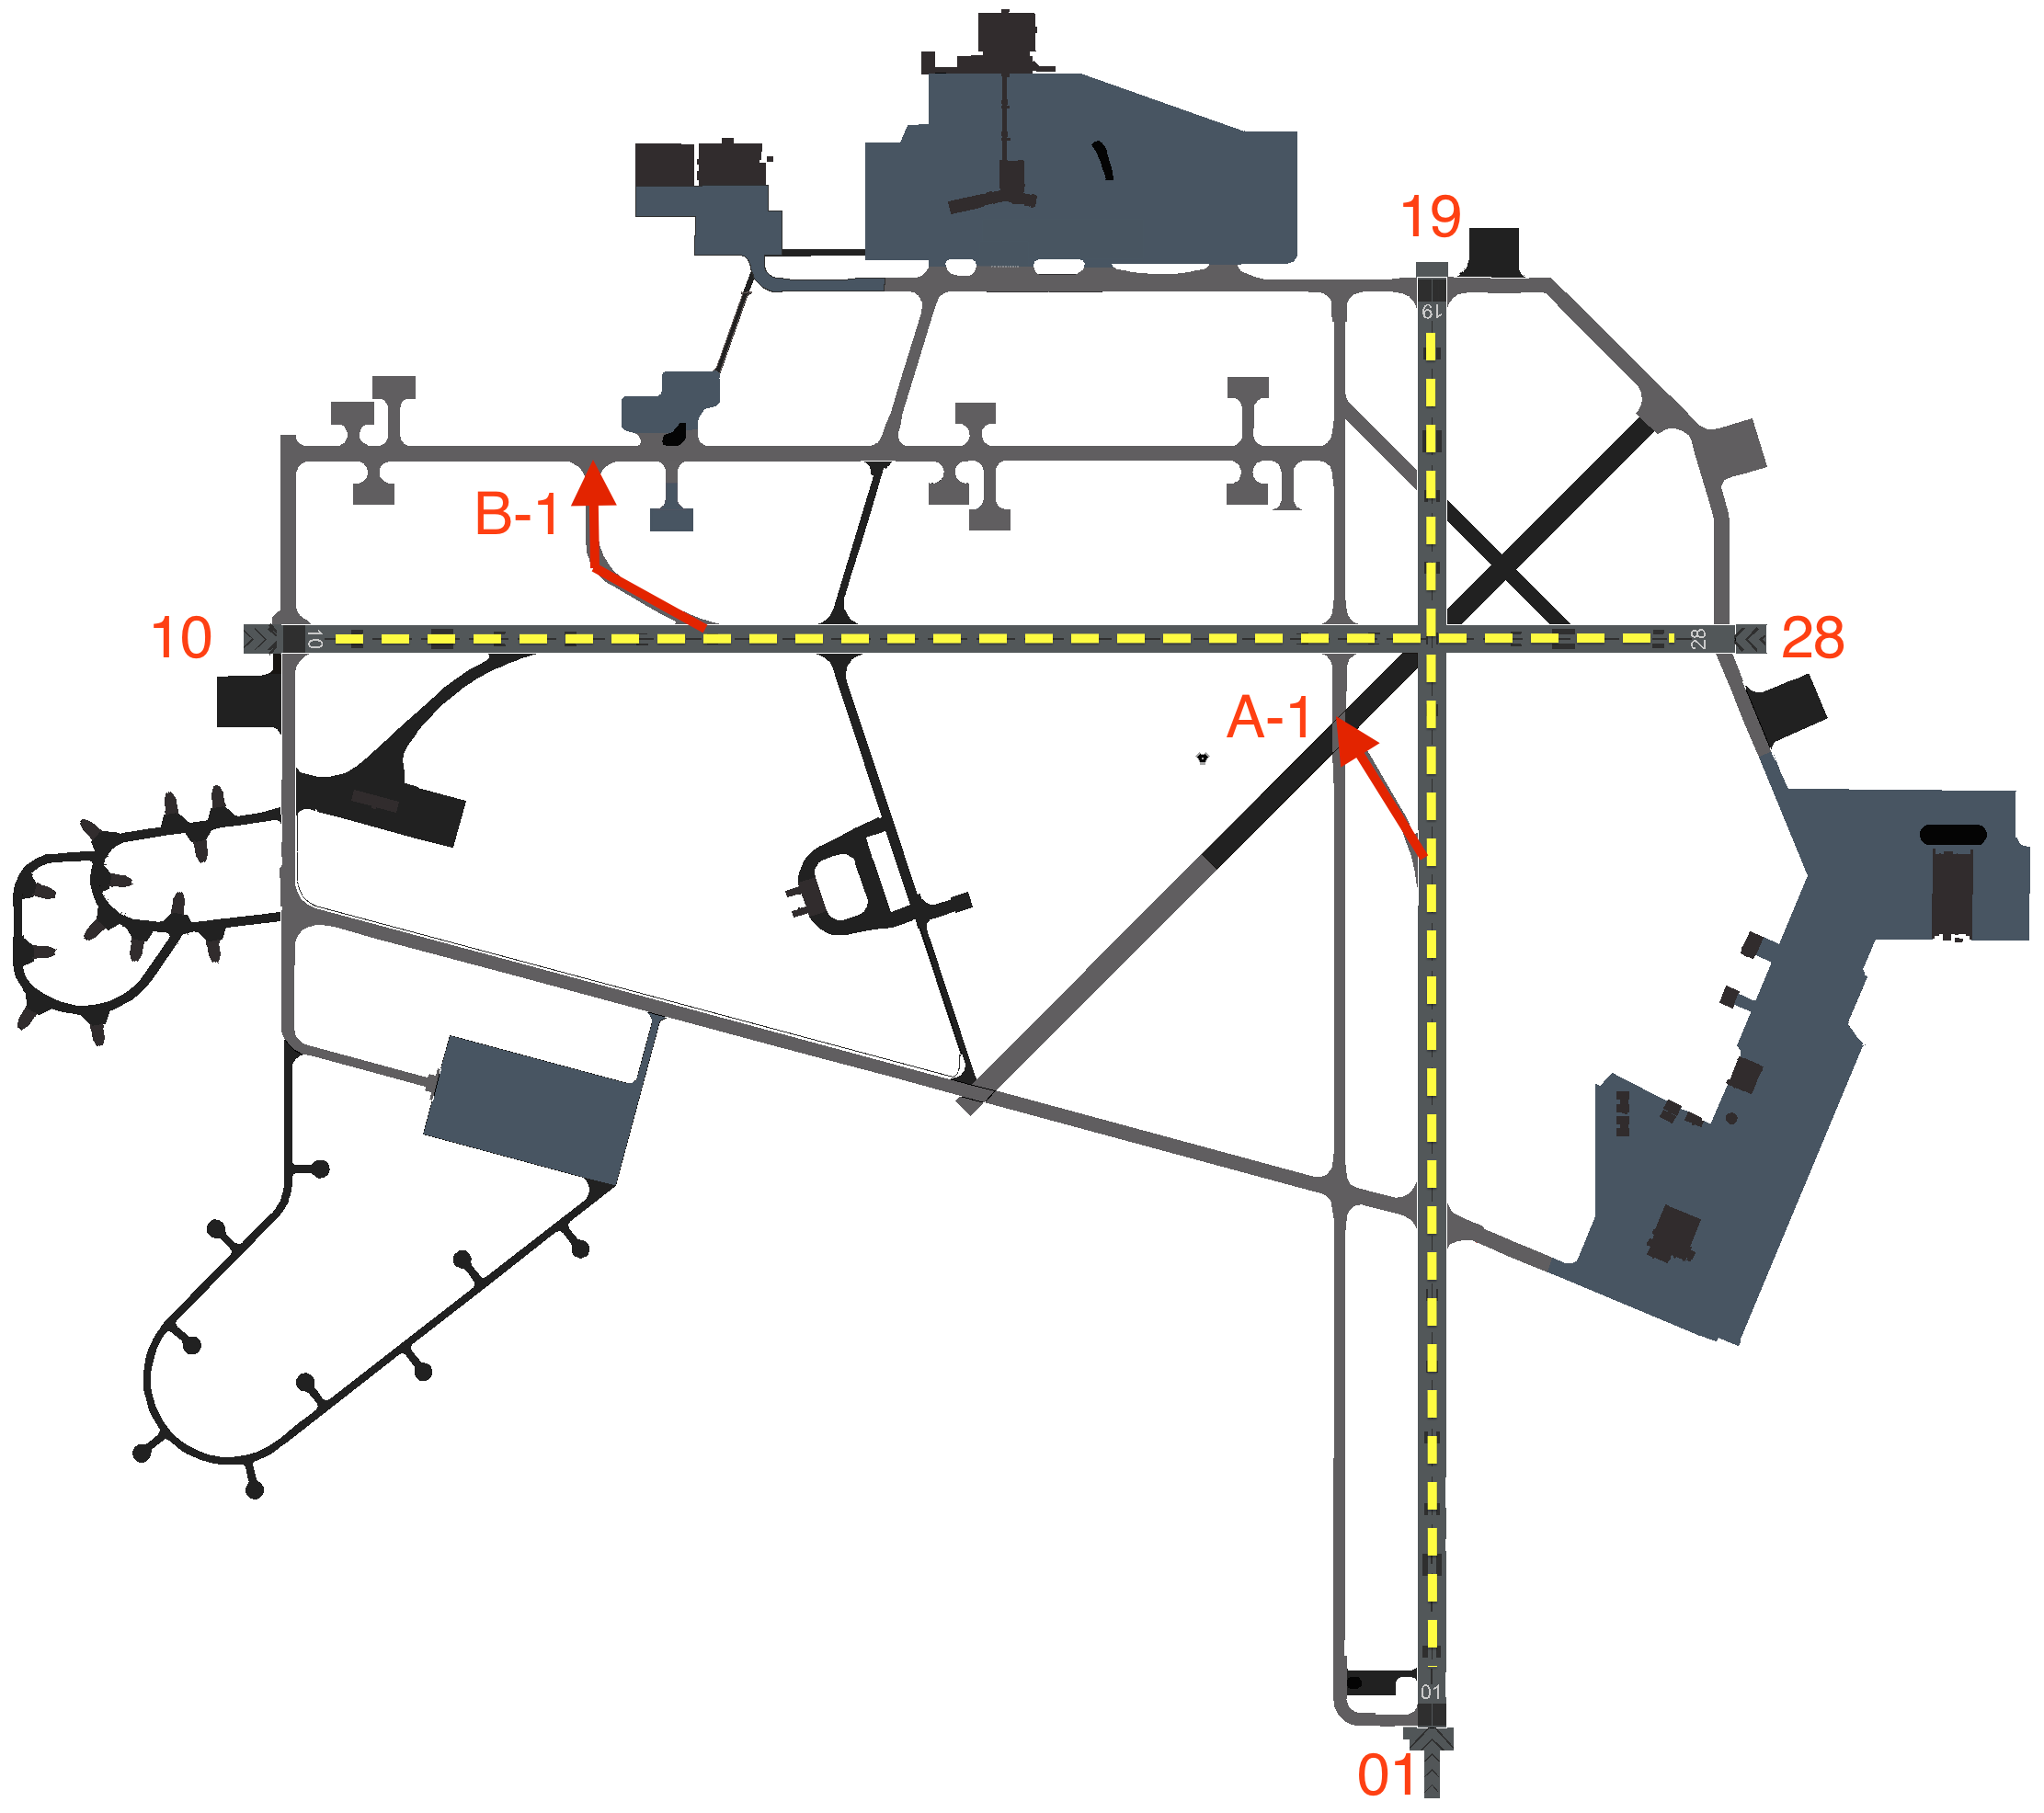
\includegraphics[width=1\textwidth]{graphics/BIKF_schematic.png}
    \caption[BIKF schematic]{BIKF schematic with four marked runways in perpendicular configuration (dashed yellow lines) and two rapid-exit taxiways (red arrows): TWY~A-1 on RWY~01 and TWY~B-1 on RWY~28 (source:~ Isavia).}
    \label{fig:BIKF_schematic}
\end{figure}

Despite the reduced AROT, RWY~28 remained the least used runway, servicing only 10,1$\%$ share of landing aircraft (Figure~\ref{fig:runway_usage_peak}). The preferred runway was RWY~19, servicing 37,8$\%$ of the arrivals. A statistical summary for all the runways is shown in Table~\ref{tab:all_RWY_AROT_stats}. The average AROT for the BIKF airfield amounted to 77,5 seconds.

\begin{table}[]
\centering
\resizebox{0.8\textwidth}{!} & \multicolumn{1}{l|}{50\%} & \multicolumn{1}{l|}{75\%} & \multicolumn{1}{l|}{max} \\ \hline
\multicolumn{1}{|l|}{RWY 01} & 1253 & 86 & 23 & 46 & 66 & 88 & 101 & 153 \\ \hline
\multicolumn{1}{|l|}{RWY 10} & 1190 & 87 & 12 & 61 & 79 & 86 & 93 & 155 \\ \hline
\multicolumn{1}{|l|}{RWY 19} & 1770 & 68 & 10 & 46 & 62 & 66 & 71 & 155 \\ \hline
\multicolumn{1}{|l|}{RWY 28} & 470 & 69 & 14 & 49 & 61 & 66 & 74 & 155 \\ \hline
\end{tabular}%
}
\caption[AROTs during peak hours by runway]{AROT statistics for the air traffic mix at BIKF during peak hours by runway. The count is the number of landings during peak hours from October 2017 to November 2018.}
\label{tab:all_RWY_AROT_stats}
\end{table}


% ---------------------------

\section{Inter-arrival Distance Separation}\label{sec:interarrival_dist_sep_RECAT}

The information for the arrival pairs was fitted into the ICAO WTC scheme in order to recognise the prevailing aircraft pair mix, which is a consequence of the traffic mix discussed previously in \ref{sec:traffic_mix}. Clearly the majority of arrival pairs were classified as Medium-Medium (M-M) as shown in Table~\ref{tab:pairs_mix_to_wtc}. The other noticeable pairs were variations of the Heavy and the Medium categories -- H-H, H-M and M-H. Those four pair types formed the subset of data to be further analysed and split into RECAT-EU categories. The rest of the pairs containing Light aircraft were discarded as being insignificant because of their limited number. 

% Please add the following required packages to your document preamble:
% \usepackage{multirow}
% \usepackage{graphicx}
% \usepackage[table,xcdraw]{xcolor}
% If you use beamer only pass "xcolor=table" option, i.e. \documentclass[xcolor=table]{beamer}
\begin{table}[h]
\centering
\resizebox{0.3\textwidth}{!}{%
\begin{tabular}{cc|r|r|r|}
\cline{3-5}
\multicolumn{1}{l}{} & \multicolumn{1}{l|}{} & \multicolumn{3}{c|}{Follower} \\ \cline{3-5} 
\multicolumn{1}{l}{} & \multicolumn{1}{l|}{} & \multicolumn{1}{c|}{H} & \multicolumn{1}{c|}{M} & \multicolumn{1}{c|}{L} \\ \hline
\multicolumn{1}{|c|}{} & H & \cellcolor[HTML]{FFCC67}56 & \cellcolor[HTML]{FE996B}334 & \cellcolor[HTML]{FFFFC7}2 \\ \cline{2-5} 
\multicolumn{1}{|c|}{} & M & \cellcolor[HTML]{FE996B}368 & \cellcolor[HTML]{FD6864}1809 & \cellcolor[HTML]{FFFFC7}7 \\ \cline{2-5} 
\multicolumn{1}{|c|}{\multirow{-3}{*}{\rotatebox[origin=c]{90}{Leader}}} & L & \cellcolor[HTML]{FFFFC7}3 & \cellcolor[HTML]{FFFFC7}9 & \cellcolor[HTML]{FFFFC7}1 \\ \hline
\end{tabular}%
}
\caption[BIKF traffic mix sorted into ICAO WTC]{Number of ICAO pairs from the traffic mix at BIKF during peak hours, arranged into the corresponding wake categories. The observation period is from October 2017 to November 2018.}
\label{tab:pairs_mix_to_wtc}
\end{table}

The ICAO WTC scheme specifies a distance separation minima as prescribed in  Table~\ref{tab:ICAO_WTC}. The distributions of the distance separations from the selected four pair-types were examined and presented in Figure~\ref{fig:dist_separ_HH_HM_MH_MM_pairs} along with the ICAO reference separation minima. 

\fxnote{Why are some data to the left of the red line???}
\begin{figure}[h]
    \centering
    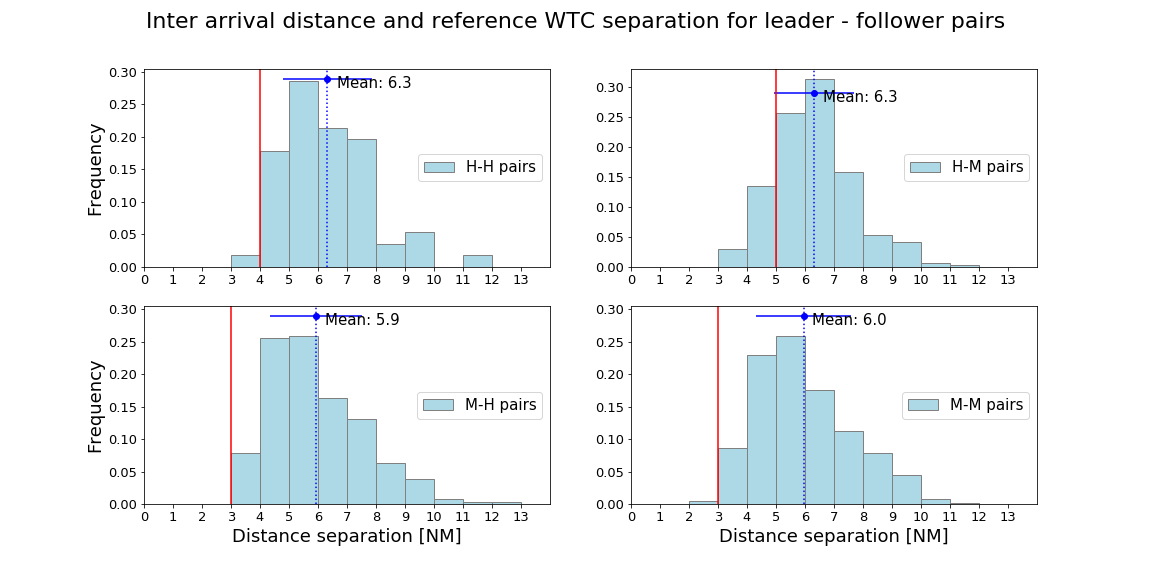
\includegraphics[width=1\textwidth]{graphics/fig_dist_separ_HH_HM_MH_MM_pairs.png}
    \caption[Distribution of distance separation for ICAO pairs]{Distribution of the WTC distance separation between selected ICAO pair categories. The red reference line indicates the separation minima for a particular pair category. The blue horizontal line indicates 1 standard deviation left and right of the mean.}
    \label{fig:dist_separ_HH_HM_MH_MM_pairs}
\end{figure}



Each of the ICAO pairs were re-categorised, the data-set was reduced by filtering out the pair categories with insufficient number of data points. The mix of arrival pairs from the peak hour traffic at BIKF after re-categorisation is presented in Table~\ref{tab:pairs_mix_to_recat}. As expected from the traffic fleet analysis in \ref{sec:traffic_mix}, most of the aircraft combined into C-C pairs. The rest of the more significant traffic pairs were variations from CAT-C, CAT-D and CAT-E categories.

% Please add the following required packages to your document preamble:
% \usepackage{multirow}
% \usepackage{graphicx}
% \usepackage[table,xcdraw]{xcolor}
% If you use beamer only pass "xcolor=table" option, i.e. \documentclass[xcolor=table]{beamer}
\begin{table}[h]
\centering
\resizebox{0.8\textwidth}{!}{%
\begin{tabular}{cc|c|c|c|c|c|c|}
\cline{3-8}
\multicolumn{1}{l}{} & \multicolumn{1}{l|}{} & \multicolumn{6}{c|}{Follower} \\ \cline{3-8} 
\multicolumn{1}{l}{} & \multicolumn{1}{l|}{} & CAT-A & CAT-B & CAT-C & CAT-D & CAT-E & CAT-F \\ \hline
\multicolumn{1}{|c|}{} & CAT-A &  &  &  & \cellcolor[HTML]{FFFFC7}1 &  &  \\ \cline{2-8} 
\multicolumn{1}{|c|}{} & CAT-B &  & \cellcolor[HTML]{FFFFC7}1 & \cellcolor[HTML]{FFFC9E}17 & \cellcolor[HTML]{FFFC9E}16 & \cellcolor[HTML]{FFFFC7}2 &  \\ \cline{2-8} 
\multicolumn{1}{|c|}{} & CAT-C &  & \cellcolor[HTML]{FFFC9E}19 & \cellcolor[HTML]{FD6864}1697 & \cellcolor[HTML]{FE996B}242 & \cellcolor[HTML]{FFCE93}41 & \cellcolor[HTML]{FFFC9E}14 \\ \cline{2-8} 
\multicolumn{1}{|c|}{} & CAT-D & \cellcolor[HTML]{FFFFC7}1 & \cellcolor[HTML]{FFFC9E}10 & \cellcolor[HTML]{FE996B}229 & \cellcolor[HTML]{FE996B}200 & \cellcolor[HTML]{FFFC9E}10 & \cellcolor[HTML]{FFFFC7}5 \\ \cline{2-8} 
\multicolumn{1}{|c|}{} & CAT-E &  & \cellcolor[HTML]{FFFFC7}1 & \cellcolor[HTML]{FFCE93}44 & \cellcolor[HTML]{FFFFC7}10 &  &  \\ \cline{2-8} 
\multicolumn{1}{|c|}{\multirow{-6}{*}{\rotatebox[origin=c]{90}{Leader}}} & CAT-F &  &  & \cellcolor[HTML]{FFFC9E}16 & \cellcolor[HTML]{FFFFC7}10 & \cellcolor[HTML]{FFFFC7}1 &  \\ \hline
\end{tabular}%
}
\caption[BIKF traffic mix sorted into RECAT-EU categories]{Number of RECAT-EU pairs from the traffic mix at BIKF during peak hours, arranged into the corresponding wake categories. The vast majority of arrival pairs are classified as C-C. The observation period is from October 2017 to November 2018.}
\label{tab:pairs_mix_to_recat}
\end{table}








The resulting pairs from the ICAO H-H pairs were re-categorised primarily as C-C (87,5\%) and C-B (10,7\%) into the RECAT-EU scheme (Table~\ref{fig:HH_to_RECAT_pairs_dist_separ}). It is apparent that for those two pairs the RECAT-EU scheme would decrease the required separation minima by one nautical mile (from 4 NM to 3 NM). The share of the H-H pairs was 2,2\% of all observed pairs at BIKF.

\begin{figure}[h]
    \centering
    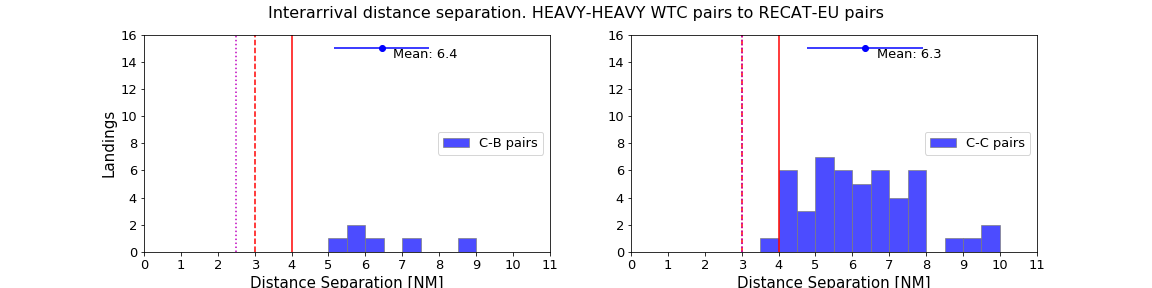
\includegraphics[width=1\textwidth]{graphics/fig_HH_to_RECAT_pairs_dist_separ.png}
    \caption[Inter-arrival distance separation of ICAO H-H pairs into the RECAT-EU scheme]{Inter-arrival distance separation after re-categorisation of ICAO H-H pairs into the RECAT-EU scheme. The vertical lines indicate the separation minima in different schemes (ICAO - solid red line, RECAT-EU - dashed red line, MRS - dotted magenta line)}
    \label{fig:HH_to_RECAT_pairs_dist_separ}
\end{figure}

For the aircraft pairs of the ICAO H-M category, the transition to the RECAT-EU scheme will decrease the separation minima requirements more significantly. The reduction for aircraft pairs that were re-categorised as B-C or B-D category is from 5 NM to 4 NM, while for the C-C and C-D pairs this reduction is 2~NM, from 5~NM to 3~NM (Figure~\ref{fig:HM_to_RECAT_pairs_dist_separ}). Here again the C-C pairs were predominant with 73,8\% and C-D pairs with 10,8\%. The share of the B-C and B-D pairs was around 5\%. Provided that the MRS requirements allow for reduced minima, the D-D pairs from the ICAO H-M pair category would potentially result in 2,5~NM reduction, but only three of those pairs were present in the observed data subset (Figure~\ref{fig:HM_to_DD_pairs_dist_separ}). The share of the H-M pair category from the whole BIKF traffic during peak hours is 12,9\%.

\begin{figure}[h]
    \centering
    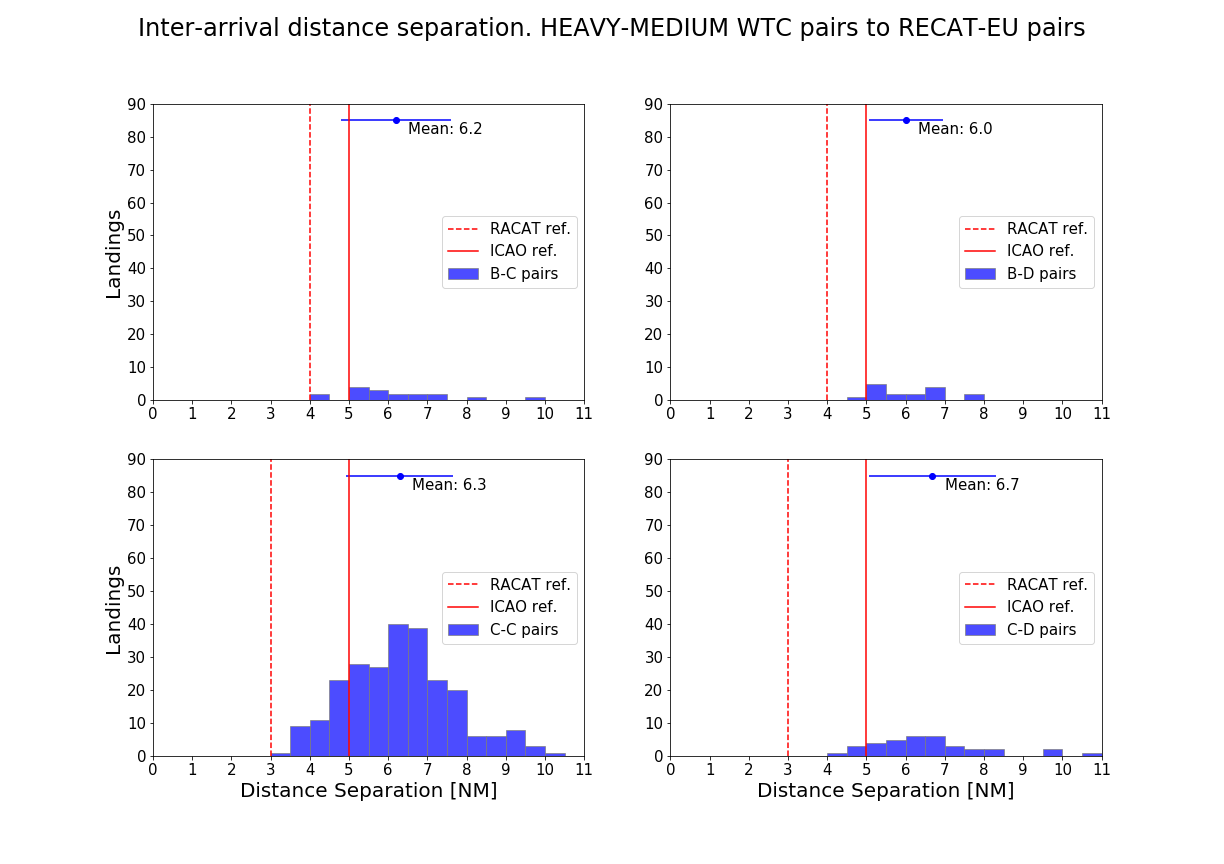
\includegraphics[width=1\textwidth]{graphics/fig_HM_to_RECAT_pairs_dist_separ.png}
    \caption[Inter-arrival distance separation of ICAO H-M pairs into the RECAT-EU scheme]{Inter-arrival distance separation after re-categorisation of ICAO H-M pairs into the RECAT-EU scheme.}
    \label{fig:HM_to_RECAT_pairs_dist_separ}
\end{figure}

The re-categorisation of  the ICAO M-H (Figure~\ref{fig:MH_to_RECAT_pairs_dist_separ}) and M-M (Figure~\ref{fig:MM_to_RECAT_pairs_dist_separ}) pairs from the data subset shows no apparent advantage for the newly formed RECAT-EU pairs. The traffic in both cases is concentrated in the C-C pairs category. The RECAT-EU reference separation minima does not change its position after re-categorisation to allow for any shift in the separation distribution between aircraft pairs. In both schemes the reference separation was specified as 3 NM, or 2,5 NM when the MRS was applicable. In the case of BIKF the MRS minima was established at 3 NM because of technical characteristics of the radar system, as mentioned earlier. The 2,5 NM dotted line in the figures was drawn just for comparison and not as a reference minima limit.  Pairs from the C-C category comprise 77,9\% of all the ICAO M-H pairs, followed by the D-C pair category with 11,4\%.

\begin{figure}[h]
    \centering
    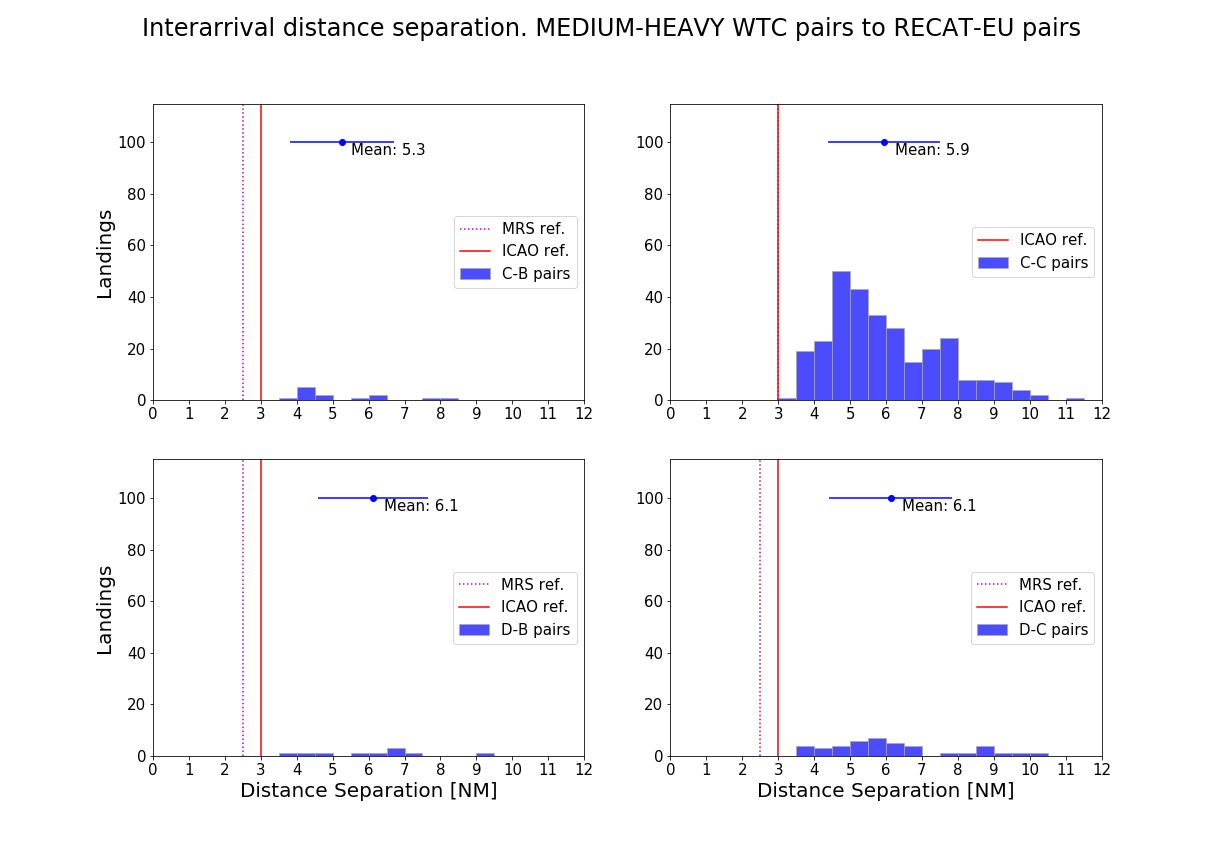
\includegraphics[width=1\textwidth]{graphics/fig_MH_to_RECAT_pairs_dist_separ.png}
    \caption[Inter-arrival distance separation of ICAO M-H pairs into the RECAT-EU scheme]{Inter-arrival distance separation after re-categorisation of ICAO M-H pairs into the RECAT-EU scheme.}
    \label{fig:MH_to_RECAT_pairs_dist_separ}
\end{figure}

The portion of C-C pairs from the last category, the M-M pairs, is also prevailing with 61,8\%, followed by the C-D (11,4\%), D-D (10,8\%) and D-C (10,4\%) pairs. The lower percentage of the C-C pairs from the ICAO M-M category in comparison with the other ICAO categories after re-categorisation was accompanied by increased ratio of the other pair categories, as noticed in the percentage values and in Figure~\ref{fig:MM_to_RECAT_pairs_dist_separ}. The reference separation minima remains unchanged after re-categorisation, similar to the M-H pairs. This result was also evidence that most of the aircraft traffic mix for Keflavík Airport were in the Medium category.

\begin{figure}[h]
    \centering
    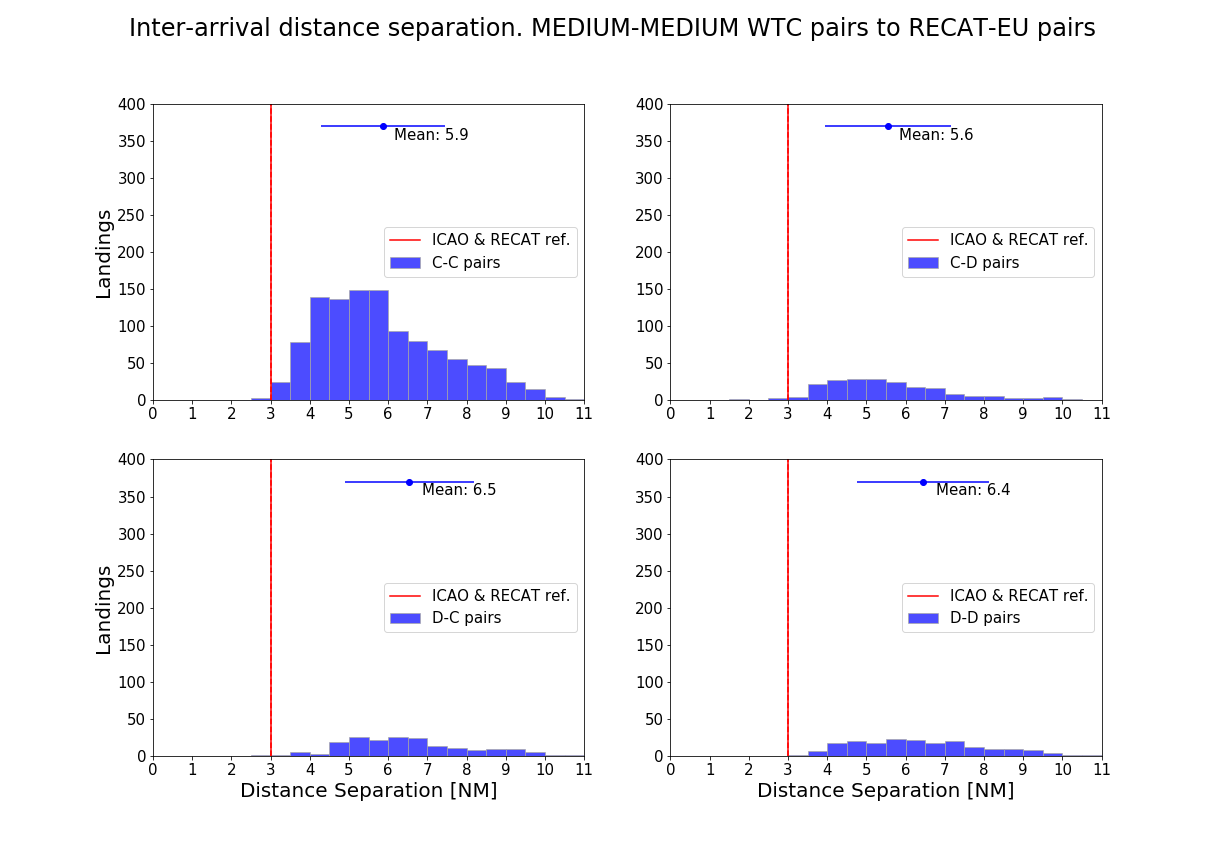
\includegraphics[width=1.0\textwidth]{graphics/fig_MM_to_RECAT_pairs_dist_separ.png}
    \caption[Inter-arrival distance separation of ICAO M-M pairs into the RECAT-EU scheme]{Inter-arrival distance separation after re-categorisation of ICAO M-M pairs into the RECAT-EU scheme.}
    \label{fig:MM_to_RECAT_pairs_dist_separ}
\end{figure}

The share of the M-H pairs from the whole BIKF traffic during peak hours is 14,3\%. The share of the M-M pairs on the other hand is the largest of all ICAO pairs - 69.8\%. The figures above were also evidence that incorporating the RECAT-EU scheme for the selected data subset, would potentially assist the aircraft pairs with a Heavy leader, but would not change the situation for pairs with a Medium leader. 

It is illustrative to mention also that some of the pair categories would suffer an increase in the separation minima in the RECAT-EU scheme. Such example from the traffic at Keflavík would be the C-F and D-F pairs from the ICAO M-M category (Figure~\ref{fig:MM_to_CF_and_DF_pairs_dist_separ}). The reference separation in the former case would double from 3 NM up to 6 NM and in the later case the increase would be from 3 NM to 5 NM. Those pairs were rare in the data set and insufficient to reach any accurate conclusion. Only two pairs from the M-M category for the selected time period were in the D-F category and eight pairs were in the C-F category.

\begin{figure}[h]
    \centering
    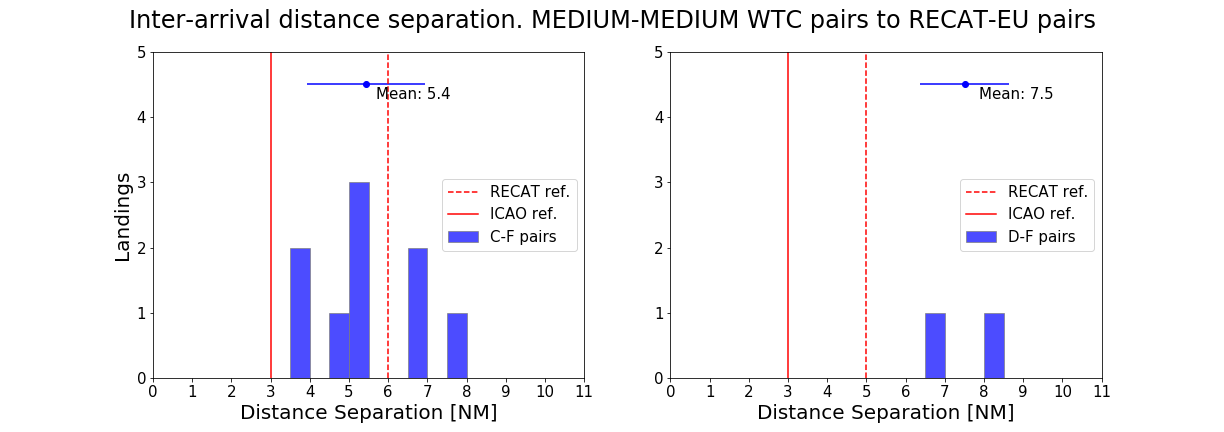
\includegraphics[width=1\textwidth]{graphics/fig_MM_to_CF_and_DF_pairs_dist_separ.png}
    \caption[Inter-arrival distance separation of ICAO M-M pairs into the RECAT-EU C-F and D-F pairs]{Inter-arrival distance separation after re-categorisation of ICAO M-M pairs into the RECAT-EU C-F and D-F pairs.}
    \label{fig:MM_to_CF_and_DF_pairs_dist_separ}
\end{figure}




\section{Landing Time Interval}\label{sec:LTI}
The method used to determine the landing time interval (LTI) requires the examination of aircraft pairs -- i.e. leader and follower. The data-set for the analysis contained the ICAO type and WTC for the leader and the follower along with distance separation and time separation between the aircraft in each pair during peak hours. The time frame was identical with the one used in the previous sections. Additionally every leader and follower were re-categorised and assigned a RECAT-EU designator.


Another important metric derived from the data, together with the distance separation between pairs, was the landing time interval (LTI) that indicates whether AROT or the separation requirement is the limiting factor for airfield capacity. As stated in the study objective \ref{sec:arot_and_study_objective} the LTI quantifies the time separation between aircraft in a pair, calculated from the distance separation and the final approach speed of the following aircraft. This measurement was computed for each of the observed pairs and is presented in Figure~\ref{fig:time_separ_HH_HM_MH_MM_pairs}, where the reference line indicates the time that a follower takes to travel the distance minima for the respective pair category. 

The final approach velocity for this calculation was set equal to the maximum average approach velocity from all four runways. This is done by finding the average velocity for each of four runways and using the maximum of the four values as the final approach velocity for the calculation of the LTI. Higher velocity value results in lower reference time. In this sense the reference time is a more liberally specified constraint, as opposed to using the minimum of the average approach velocities. Similar methodology is currently being used by Isavia in determining the runway capacity envelope.

\begin{figure}[h]
    \centering
    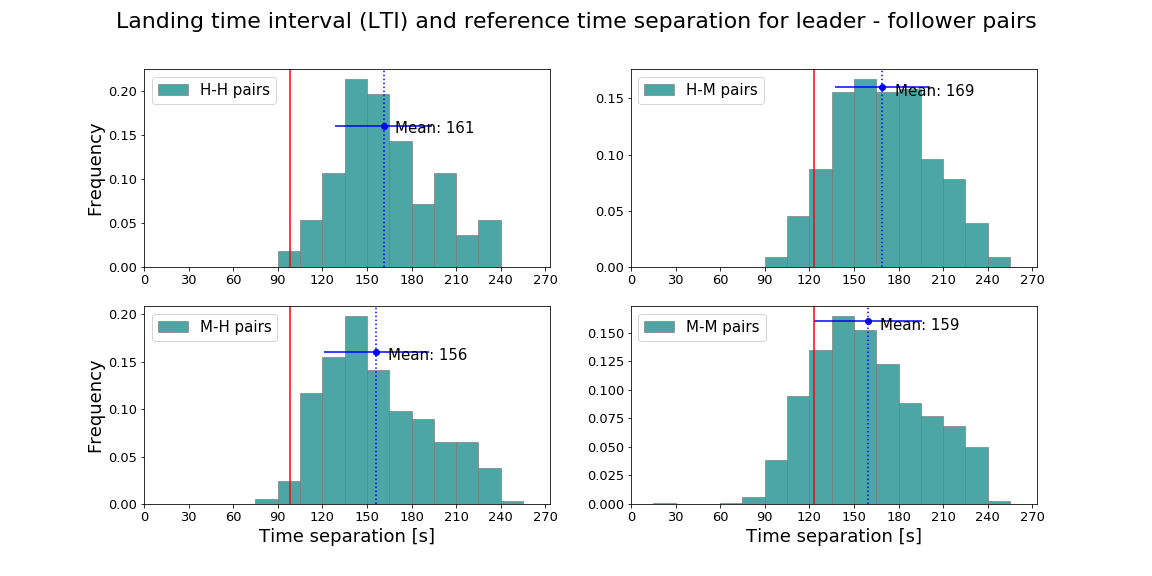
\includegraphics[width=1\textwidth]{graphics/fig_time_separ_HH_HM_MH_MM_pairs.png}
    \caption[Distribution of landing time interval (LTI) for ICAO pairs]{Distribution of of landing time interval (LTI) for selected ICAO pair categories. The red line indicates a liberal time reference estimate for a particular pair category. The blue horizontal line indicates 1 standard deviation left and right of the mean.}
    \label{fig:time_separ_HH_HM_MH_MM_pairs}
\end{figure}



\section{Constraints for Increased Capacity}% Runway Occupancy and Landing Time Interval for RECAT-EU pairs}

The following section presents the landing time intervals (LTI) for a subset of data points after re-categorisation from the ICAO wake turbulence scheme. The subset contained primarily C-C pairs. The C-C pairs were selected on the basis of being the more prominent subset with most of the data points. The LTI for the ICAO pair sets from \ref{sec:LTI} were modified to represent only the C-C pairs, where the effect on the LTI distribution after re-categorisation would be more accurate. The other metric used in contrast to the LTI was the arrival runway occupancy time for the respective aircraft pairs. The frequency distribution of the AROT included the runway occupancy for all the leaders of the selected ICAO category in order to make use of more data points and obtain a more general view on the AROT distribution. This decision was based on the assumption that the AROT of the leader in an aircraft pair is the constraint for the time separation of follower. This is illustrated in the result for the LTI and the AROT for the C-C pairs from H-H pair category in Figure~\ref{fig:CC_from_HH_pairs_time_sep}. 

\begin{figure}[h]
    \centering
    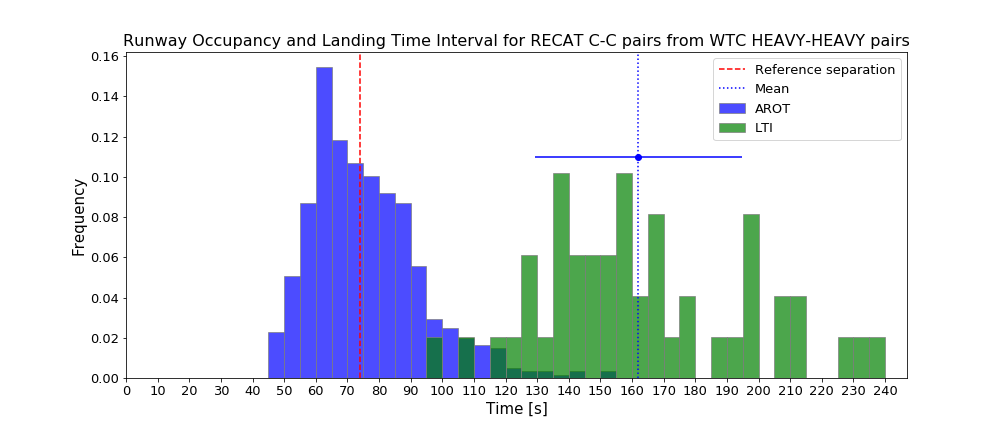
\includegraphics[width=1\textwidth]{graphics/fig_CC_from_HH_pairs_time_sep.png}
    \caption[AROT and LTI of C-C pairs originating from ICAO H-H pairs]{AROT and landing time intervals of C-C pairs originating from ICAO H-H pairs. The dashed red line indicates the RECAT-EU reference time separation for the C-C pairs. The blue horizontal line indicates 1 standard deviation left and right of the mean.}
    \label{fig:CC_from_HH_pairs_time_sep}
\end{figure}

The LTI frequency distribution contained all C-C pairs originating from the ICAO H-H category. The reference time separation (red dashed line) was calculated from the final approach speed and the RECAT-EU distance separation, as explained in \ref{sec:LTI}. The frequency distribution for the AROT, on the other hand, contained all pairs with CAT-C leader originating from the Heavy category, not only pairs with CAT-C leader and CAT-C follower. In this sense the distribution for the AROT was based on more data points than the distribution for the LTI and gave a more accurate presentation of the runway occupancy. Figure~\ref{fig:CC_from_HH_pairs_time_sep} represents the case for 1,9\% of all arrival pairs at BIKF for the observed period during peak hours.

The share of C-C pairs originating from the ICAO H-M category from the peak traffic at the airport was 9,5\%.  The LTI frequency distribution of those pairs is shown in Figure~\ref{fig:CC_from_HM_pairs_time_sep}. Here again the AROT distribution was based on the runway occupancy of CAT-C leaders, as in the previous case. 
 
\begin{figure}[h]
    \centering
    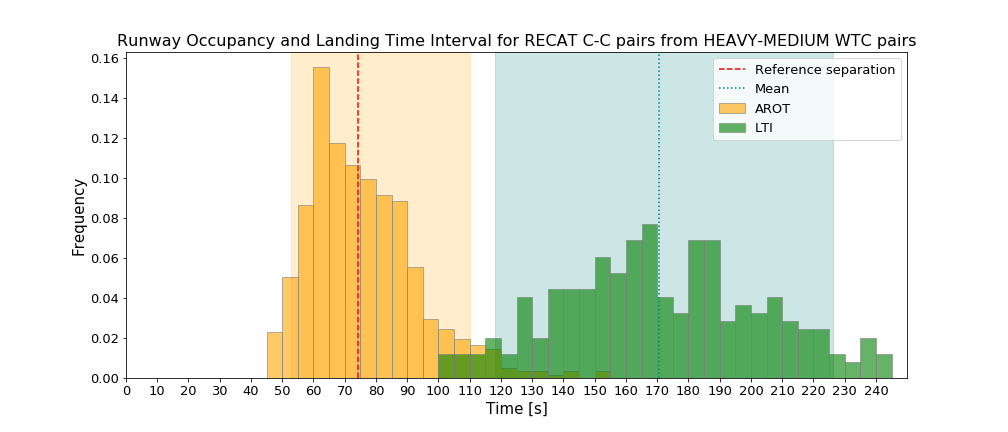
\includegraphics[width=1\textwidth]{graphics/fig_CC_from_HM_pairs_time_sep.png}
    \caption[AROT and LTI of C-C pairs originating from ICAO H-M pairs]{AROT and landing time intervals of C-C pairs originating from ICAO H-M pairs. The dashed red line indicates the RECAT-EU reference time separation for the C-C pairs. The blue horizontal line indicates 1 standard deviation left and right of the mean.}
    \label{fig:CC_from_HM_pairs_time_sep}
\end{figure}

These two cases: C-C pairs from ICAO H-H and H-M categories, would have more noticeable beneficial effect from the implementation of the RECAT-EU scheme (refer to~\ref{sec:interarrival_dist_sep_RECAT}). The decrease in distance separation in those cases is 1 NM or 2 NM. Translating the separation into the time domain resulted in a separation reference time line at 74 seconds and minimum LTI values close to 100 seconds. This shift of the reference line creates the potential for shift to the left in the frequency distribution of the LTI.
 
 \begin{figure}[h]
    \centering
    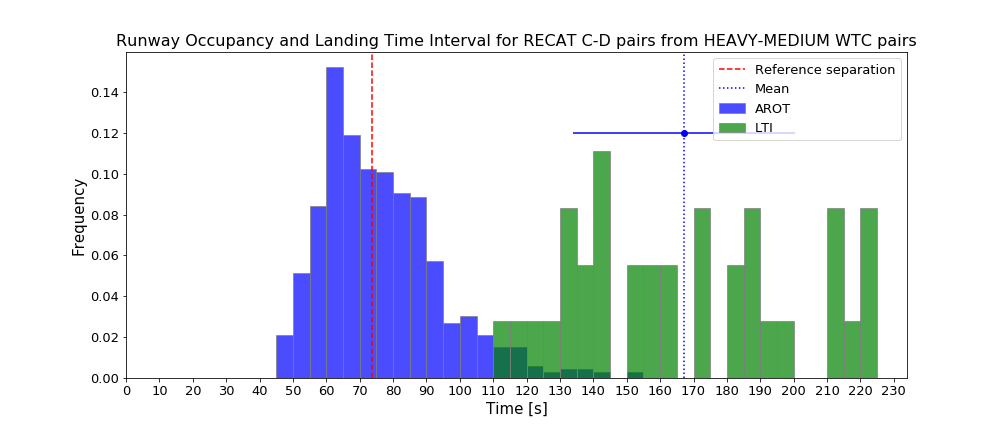
\includegraphics[width=1\textwidth]{graphics/fig_CD_from_HM_pairs_time_sep.png}
    \caption[AROT and LTI of C-D pairs originating from ICAO H-M pairs]{AROT and landing time intervals of C-D pairs originating from ICAO H-M pairs. The dashed red line indicates the RECAT-EU reference time separation for the C-D pairs. The blue horizontal line indicates 1 standard deviation left and right of the mean.}
    \label{fig:CD_from_HM_pairs_time_sep}
\end{figure}

Even greater potential for decrease of the inter-arrival time was observed in the case of C-D pairs from the ICAO H-M category (Figure~\ref{fig:CD_from_HM_pairs_time_sep}). Here the minimum LTI observed was 113 seconds, serving as a possible 39 seconds shift to the left of the frequency distribution. However the share of those pairs in the traffic was limited to 1.4\%.

The C-C pairs formed from the ICAO M-H category were 11,1\% from the BIKF traffic with frequency distribution of the LTI shown in Figure~\ref{fig:CC_from_MH_pairs_time_sep}. The reference line in this case is again at 74 seconds, and the LTI frequency distribution curve was closer to the reference than in the cases above.

\begin{figure}[h]
    \centering
    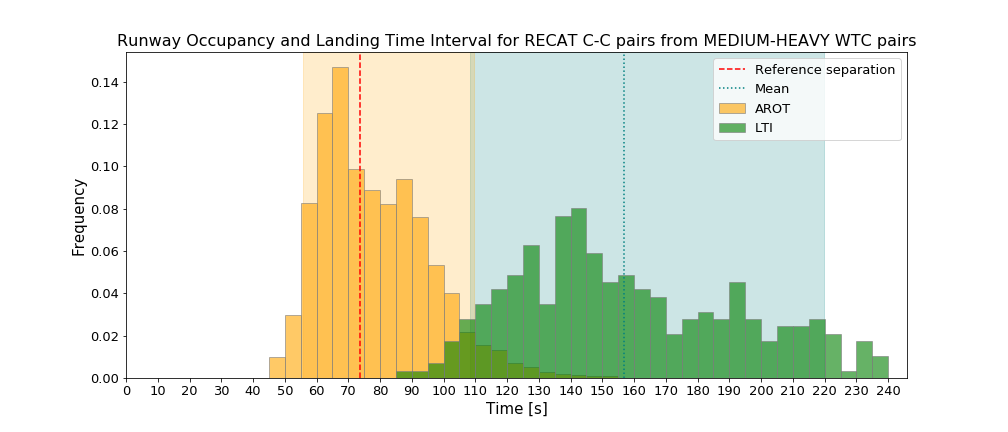
\includegraphics[width=1\textwidth]{graphics/fig_CC_from_MH_pairs_time_sep.png}
    \caption[AROT and LTI of C-C pairs originating from ICAO M-H pairs]{AROT and landing time intervals of C-C pairs originating from ICAO M-H pairs. The dashed red line indicates the RECAT-EU reference time separation for the C-C pairs. The blue horizontal line indicates 1 standard deviation left and right of the mean.}
    \label{fig:CC_from_MH_pairs_time_sep}
\end{figure}

The majority of the C-C pairs of the BIKF traffic were formed from the ICAO M-M pairs, or 43\%. Here the minimum inter-arrival time separation was 80 seconds, a mere 6 seconds above the reference limit, with half of all pairs having LTI between 132 and 185 seconds.

\begin{figure}[h]
    \centering
    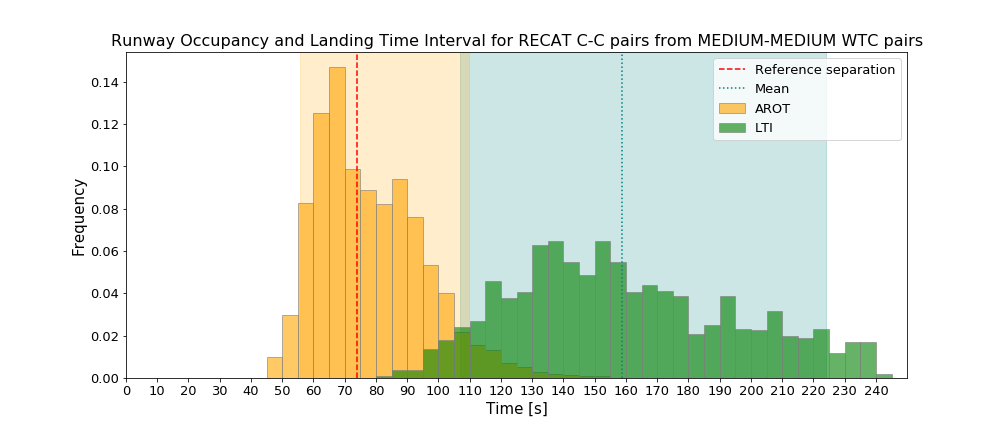
\includegraphics[width=1\textwidth]{graphics/fig_CC_from_MM_pairs_time_sep.png}
    \caption[AROT and LTI of C-C pairs originating from ICAO M-M pairs]{AROT and landing time intervals of C-C pairs originating from ICAO M-M pairs. The dashed red line indicates the RECAT-EU reference time separation for the C-C pairs. The blue horizontal line indicates 1 standard deviation left and right of the mean.}
    \label{fig:CC_from_MM_pairs_time_sep}
\end{figure}

Nevertheless the potential for decrease of the landing time interval was hindered by the AROT, the other major factor affecting runway capacity (refer to \ref{sec:runway_capacity}). All of the distributions in the figures above witness an overlap of the reference time separation line and the AROT frequency distribution. The average runway occupancy time was estimated as 77,5 seconds (\ref{ssec:runway_usage_arot}) and compared to the reference time line for the predominant C-C pairs (74 seconds), it is apparent that the AROT is the limiting factor and a major constraint for shift in the LTI distribution.








% \lipsum[28-34]

%%% Local Variables: 
%%% mode: latex
%%% TeX-master: "DEGREE-NAME-YEAR"
%%% End: 
